\documentclass{article}
\usepackage[utf8]{inputenc}

\title{Ph20 Problem Set #3}
\author{Morgaine Mandigo-Stoba}
\date{Section 1}

\usepackage{natbib}
\usepackage{graphicx}
\usepackage{physics}

\begin{document}

\maketitle

\section{Part 1}

\subsection{Explicit Euler Simulation}

\begin{figure}[h!]
\centering
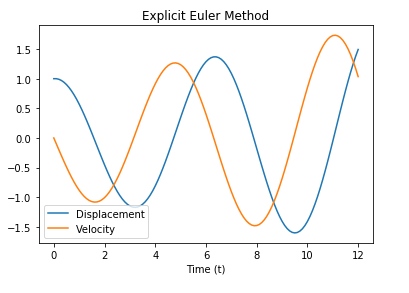
\includegraphics[scale=0.35]{exp_euler.png}
\caption{Plot of position and velocity over time generated with the Explicit Euler Method and a time step of 0.1}
\label{fig:expeuler}
\end{figure}

\subsection{Explicit Euler Error}

The analytic solution to this problem is $x=cos(x)$ and $v=-sin(x)$. 

\begin{figure}[h!]
\centering
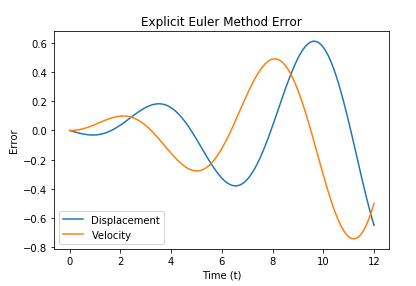
\includegraphics[scale=0.35]{exp_euler_err.png}
\caption{Plot of error in position and velocity over time of the Explicit Euler Method as compared to the analytic solution.}
\label{fig:expeulererr}
\end{figure}

\subsection{Explicit Euler Error vs Time Step}

\begin{figure}[h!]
\centering
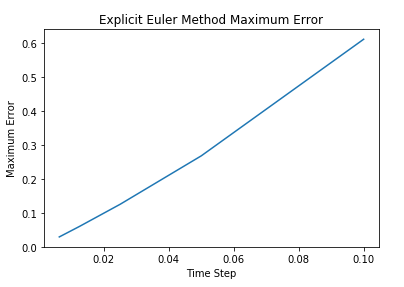
\includegraphics[scale=0.35]{exp_euler_max_err.png}
\caption{Plot of error maximum error in the Explicit Euler Method as a function of time step. The plot is very close to linear, suggesting that error is proportional to the time step for small h.}
\label{fig:expeulermaxerr}
\end{figure}

\subsection{Explicit Euler Energy}

\begin{figure}[h!]
\centering
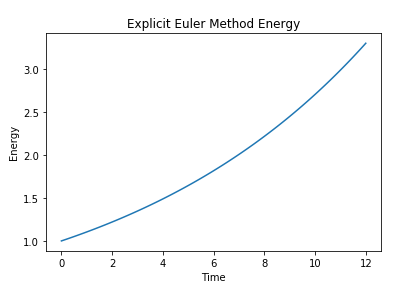
\includegraphics[scale=0.35]{exp_euler_energy.png}
\caption{Plot of error energy over time as calculated by the Explicit Euler Method. The energy clearly increases over time, on the same scale as the error.}
\label{fig:expeulerenergy}
\end{figure}

\subsection{Implicit Euler Method}

We are given the equation 
$$
    \mqty(1 & -h \\ h & 1) \mqty(x_{i+1} \\ v_{i+1}) = \mqty(x_{i} \\ v_{i})
$$
We can easily solve this by inverting the leftmost matrix, which we'll call A, and left-multiplying it on both sides. $det(A) = 1 +h^2$, so 
$$
\frac{A}{det(A)} = \mqty(\frac{1}{1 + h^2} & \frac{-h}{1 + h^2} \\ \frac{h}{1 + h^2} & \frac{1}{1 + h^2})
$$
Flipping the diagonal elements and negating the off-diagonal elements, we have
$$
A^{-1} = \mqty(\frac{1}{1 + h^2} & \frac{h}{1 + h^2} \\ \frac{-h}{1 + h^2} & \frac{1}{1 + h^2}) = \frac{1}{1 + h^2} \mqty(1 & h \\ -h & 1)
$$
Left multiplying this on both sides of the equation, we find
$$
\mqty(x_{i+1} \\ v_{i+1}) = \mqty(\frac{x_{i} + h v_{i}}{1 + h^2} \\ \frac{v_{i} - h x_{i}}{1 + h^2})
$$
And therefore our equations are
$$
x_{i+1} = \frac{x_{i} + h v_{i}}{1 + h^2} \space and \space v_{i+1} = \frac{v_{i} - h x_{i}}{1 + h^2}
$$

\begin{figure}[h!]
\centering
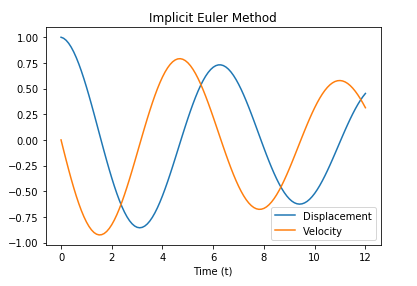
\includegraphics[scale=0.35]{imp_euler.png}
\caption{Plot of position and velocity over time generated with the Implicit Euler Method and a time step of 0.1}
\label{fig:impeuler}
\end{figure}

\begin{figure}[h!]
\centering
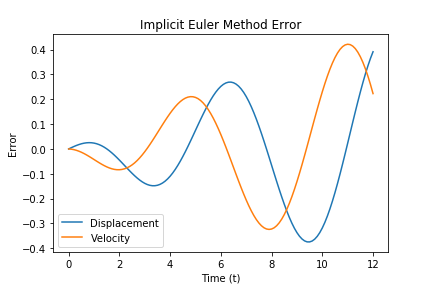
\includegraphics[scale=0.35]{imp_euler_err.png}
\caption{Plot of error in position and velocity over time of the Implicit Euler Method as compared to the analytic solution.}
\label{fig:impeulererr}
\end{figure}

\begin{figure}[h!]
\centering
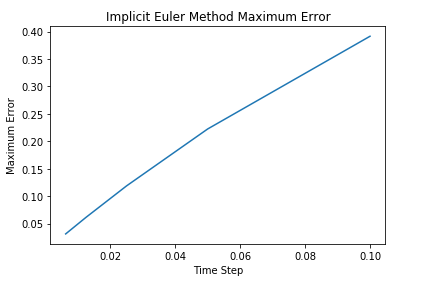
\includegraphics[scale=0.35]{imp_euler_max_err.png}
\caption{Plot of error maximum error in the Implicit Euler Method as a function of time step. The plot is very close to linear, suggesting that error is proportional to the time step for small h.}
\label{fig:impeulermaxerr}
\end{figure}

\begin{figure}[h!]
\centering
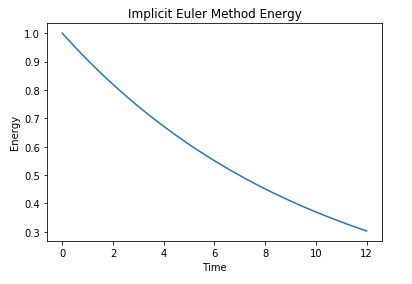
\includegraphics[scale=0.35]{imp_euler_energy.png}
\caption{Plot of error energy over time as calculated by the Implicit Euler Method. The energy clearly decreases over time, on the same scale as the error increases.}
\label{fig:impeulerenergy}
\end{figure}

\break

\section{Part 2}


\subsection{Phase Space Geometry of Explicit and Implicit Euler}

\begin{figure}[h!]
\centering
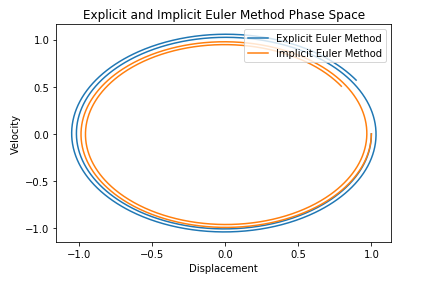
\includegraphics[scale=0.35]{exp_imp_phase.png}
\caption{Phase space plot of Explicit and Implicit Euler Methods with a time step of 0.01. Note that neither method produces a closed figure.}
\label{fig:expimpphase}
\end{figure}

\subsection{Phase Space Geometry of Symplectic Euler Method}

\begin{figure}[h!]
\centering
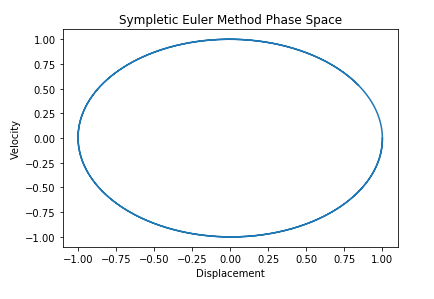
\includegraphics[scale=0.35]{symp_phase.png}
\caption{Phase space plot of Symplectic Euler Method with the same time step of 0.01 as the previous plot. Unlike the previous plot, this figure is closed.}
\label{fig:sympphase}
\end{figure}

\subsection{Symplectic Euler Method Energy}

\begin{figure}[h!]
\centering
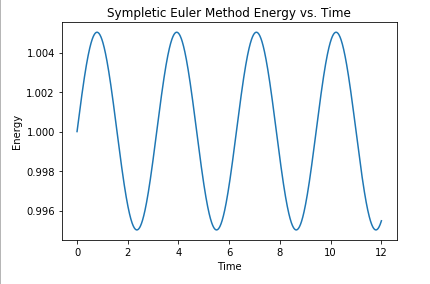
\includegraphics[scale=0.35]{symp_energy.png}
\caption{Plot of energy of the Symplectic Euler Method over time. The energy oscillates with very small amplitude around the actual value with no large-scale increase or decrease. This is consistent with this approximation being much closer to the true solution as demonstrated by the closed figure in the previous phase-space plot.}
\label{fig:sympenergy}
\end{figure}

\end{document}
